\documentclass{article}
\usepackage{graphicx}
\usepackage[margin=1.5cm]{geometry}
\usepackage{amsmath}

\begin{document}

\title{Monday Reading Assessment: Unit 4, Forces}
\author{Prof. Jordan C. Hanson}

\maketitle

\section{Chapter 4 - Forces}

\begin{enumerate}
\item 
\begin{figure}[ht]
\centering
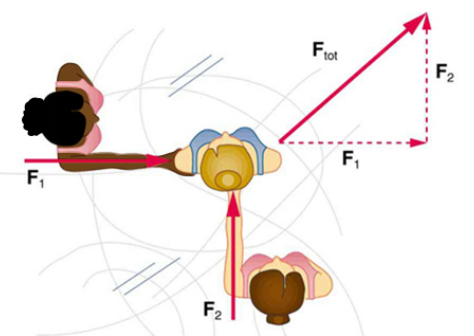
\includegraphics[width=0.4\textwidth]{skaters.png}
\caption{\label{fig:skate} Two girls push a third while skating on ice.}
\end{figure}
According to Fig. \ref{fig:skate}, a girl pushes her friend in the middle with force $\vec{F}_1 = 10\sqrt{3}\hat{i}$ N.  A second girl pushes with $\vec{F}_2 = 10\hat{j}$. (a) What is the magnitude of the net force?  (b) In what direction is the net force? \\ \vspace{3cm}
\item Will the girl being pushed move at constant velocity?  Why or why not? \\ \vspace{2cm}
\item Suppose an object is hanging from a rope, and being pulled upward with a \textbf{constant velocity} of 1.0 m/s.  The object has a weight force of 40.0 N.  (a) With what force is it being pulled?  (b) Suppose we move upwards at 1.0 m/s.  What do we perceive the velocity of the object to be?
\end{enumerate}

\end{document}
